\chapter{VESC}
\label{chap:VESC}

%\section{Funcions del VESC}

El vesc en un projecte d'opensofware i openhardware que en permet tenir un controlador de motor brushless dissenyat per a patinets elèctrics, el que ens és perfecte per controlar un motor per la nostra aplicació, a part en donar l'opció d'analitzar-lo internament

\section{Funcions del microcontrolador del VESC}

El microcontrolador tindrà emmagatzemades una sèrie de paràmetres per establir la configuració de funcionament sobre el motor, a més de paràmetres que també controlen la bateria. També disposa de diverses formes d'entrades per indicar paràmetre com el gas, sentit o extreure informació. La seva tasca és, donades les entrades designades com el gas i el sentit, determinar quins són els transistors i a quina freqüència cal generar la PWM  per tal de controlar el motor amb la màxima eficiència i generar el moviment, respectant els límits de temperatura, intensitat i voltatges tant del motor com de la bateria. 
% ??? QUIENTIO? BRUNET
%el micontrolador tinda etmagasandes una seria de paramentres del motor en quientio que podrem configurar amb la seva eina i tot de paramnes de control de la baterya. tembe disposa de vaires forma de entradas per indicar parametres com el gas sentit o extreura informacio, la seva tasca es donades les entrades designades com el gas i sentit, determinar quins transistors i a quina frequencia genera la pwm per tal de controlar el motor amb la maxima eficacia i generar el moviment, tot i respactant limits de temperatura intencitat i voltages tan del motor com de la baterya per fero de la foma mes segura 
    
\subsection{Control de la intensitat}

Un dels paràmetres principals a controlar és la intensitat. La intensitat és el factor que si es surt dels paràmetres adients pot provocar problemes en cremar components. Controlarem la intensitat mitjançant el control PWM de cada un dels transistors i mesurant la intensitat de cada fase per tal de no passar corrent en cap d'elles. A part porta intensitat màxima de drenatge de la bateria per tal de no superar els límits de la mateixa i per separat el controli intensitat màxima que pot extreure del motor cap a la bateria, per tal de mantenir el control del corrent en límits segurs. Això és degut a que les bateries tenen una capacitat molt més gran de donar corrent que de recuperar-la, a part de tot d'harmònics que poden aparèixer i pujada de voltatge en la bateria, donant-se una falsa sensació de tenir més bateria del compte. Aquest paràmetre ens permet regular-ho segons el voltatge de la bateria. Per exemple només donar corrent quan la bateria es troba més baixa d'un valor X o no donar més de XA per sobre de X.
%un del sparamentres prisiplas a controlar ja que es el que proba la magor part dels problemas de cremar els components. controlarem la intencitat mitgensant el control pwm de cada un dels mosfet i mesuran la intencitat de cada fase per tal de no pasasa de corrent en cap dellas, apat porte intencitat maxima de drenatge de la baterya per tal de no suparar els limits de la mateixa i per saparat el controli intencitat maxima que pot extreure del motor cap a la baterya per tal de mantanir el contol de la coorent en limits segus. axo es debut a que les bateryas tenen un capcasitat molt mes gran de donar corrent que de recuperarla apart de tot de ermoics que en poden apareixa i pugada de voltage en la baterya donanse una false sensacio de tenir mes baterya del conte, aqut paramente ens perment regularlo segons el voltage de la baterya per etgemple domes donnar corrent cune esta mes vaixa de X o no donan mes de XA per sobre de X, 
 
Tenir en compte que el control pot extreure corrent de la bateria emmagatzermar-la en els condensadors d'alimentació donant més intensitat al motor de la que pot extreure de la bateria durant petits períodes de temps. Per això és obligatori configurar el motor i la bateria en les intensitats corresponents, encara que siguin diferents.    
%teni en conte que el controlar pot extreure corrent de la bterya i emagamale en els condesadors de alimentacio donan mes intenciat el moto de la que pot extreure de la baterya durant pocs periodes de tems, per aixo es obligatori configurar el motor i la baterya en les intencitat corespoents. encara que sigin difarents. 
    
\subsection{Control de rampes}
En els motors elèctrics un dels principals inconvenients en el que ens trobem és que tenen un par de força pràcticament instantani. Això ens pot donar una experiència de conducció brusca i incòmoda. Per això el microcontrolador el que fa és definir un temps progressiu d 'arrancada i frenada per arribar al valor determinat. Quan més gran sigui el temps més trigarà a aconseguir la potència requerida i la conducció es farà més suau. Conforme baixi aquest temps, la conducció serà més agressiva. 
%en els motorn electric un dels inconvients que en trobem en el notre cas es que tenean un par force practicament instantani i axo ens pot doner una experiencia de conducio brusca e incomode. per axo el micocontroldor el que fa es defienir un tems progresis de arencada i frenada per arivar el valor detarmintat cuan mes gran es el tem mes tardara a consegir la poencia requeria i la conducio es fara mes suau i cuent meson tems mes \newline agresiva sera la conducio \bigskip

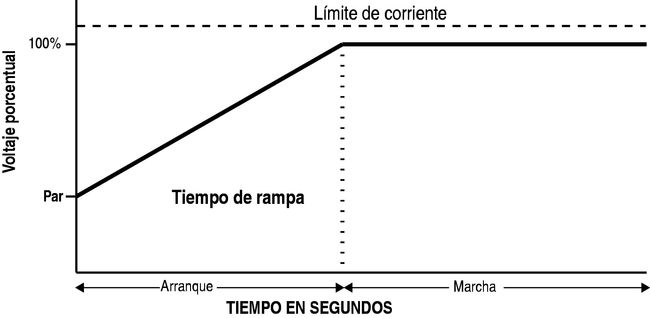
\includegraphics[width=\textwidth]{rampa}

Això es pot complicar empalmant múltiples rampes per RPM permetent oferir una corba de potència per millorar l'eficàcia del motor i la seva autonomia. Es basa en determinar unes potències a unes determinades revolucions i poder adaptar com vulguem la corba de potència.

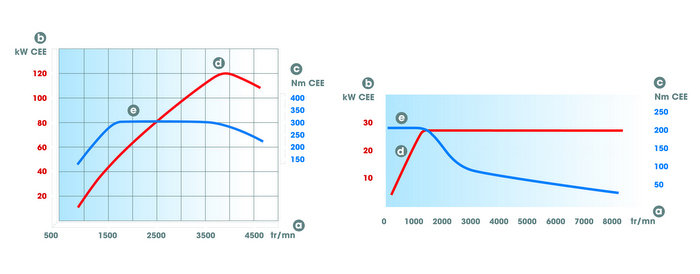
\includegraphics[width=\textwidth]{Motors/curves}

La corba de potència típica d'un motor de combustió dièsel i un motor elèctric, el disposar d'una corba tan plana ens permet jugar amb aquestes variables per tal d'emprar el par més eficient del motor i millorar l'eficiència general del vehicle, de forma que anem a buscar la corba d'un dièsel en la part eficient del nostre motor o busquem algun altra característica desitjada. En el cas de la frenada regenerativa també podem programar una corba de la intensitat que volem prenar per RPM i així millorar l'experiència de conducció.
%corba de potencia tipica de un motor de explosio disel i un motor elecric, el diposar de una corba tan plana podem gugar amb aquetas veirables per tal de utilisar la par mes eficent del motor i millorar el eficencia genaral del veicle de forma que anem a bucar la corva de un diesel en la part aficent del nostre motor o busquem alguna altre caracteritica desitgada, en el can de les frenades regenerativa tambe podem programenr un corba de la intenciat que volem drenar per RPM i axi millorar la expereincia de conducio\bigskip

\subsection{Control de la potència i les revolucions}

Podem configurar el nombre de Watts que podem injectar al motor o d'amperes per fer treballar el motor en un rang determinat, podent-lo controlar per no sobrepassar-se de potència i cremar-ho. Igual que limitar la potència total del motor, aquests paràmetres són absoluts ja que després amb les corves de potència podem reajustar-ho. Aquests valors absoluts es consideren els màxims. Ajustant la freqüència, és a dir, les revolucions del camp elèctric que li enviem al motor per tal de limitar les revolucions del motor i no sobrepassar uns límits. Per defecte i construcció tenim un límit de 50KHz en aquest driver.
%podem configurar el nobre de wats que podem igectar el motor o de ampers per la de ferlo treballar en un rang determintat i poderlo controlar per no sbobrepasarnse de potencia i cremarlo, ijual que limitar la potencia total del motor, aquts paramentres son absuluts ja que depres amb les corves de potencia podem reagustalos i ens el podem pendre com a maxims, tambe podem agustar el nombre de Hz es a dir las rebolucions del camp electric que li enviem al motor per tal de limitar les rebolucions del motor i no sobreparar un limits, per defecta i contrucio tenim un limit de 50khz en aquest driver \smallskip

\subsection{Control de temperatures}

En tot vehicle elèctric els components que gestionen la potència dissipen un percentatge d'energia en calor, i cal tenir-ho en compte per a no sobreescalfar components. Tenim l'opció de muntar un sensor de temperatura en el motor i es controla igual que amb els sensors interns.
%en tot veicle electric els compnenets que gestionen la potencia en disipan part en forma de calor i sa de tenir en conte per no sobrecalantar components, tenimm la ocio de montar senseor de temperature en el motor i controlo ijual que fariem amb els interns,

El control de temperatura ens pèrmet definir unes temperatures llindar per tal d'activar o desactivar ventiladors com a primera mesura de control. Una vegada seguim pujant de temperatura ens apareix l'opció de rampes limitadores, és a dir, unes rampes que van de la potència màxima a 0 en funció dels graus del dispositiu o el motor, limitant el seu consum de potència i evitant que s'escalfi més. És a dir podem dir que el motor de 100º a 150º vagi baixant la potència de 50Kw a 0Kw, això voldrà dir que a 120º el motor tindrà un màxim de 30Kw.
%el control de temperatura en perment defirn unas temperatura llindar per tal de activar o desactivar ventiladors com a primera mesura de control. una vegada segim pugat de tempratura ens aparaex la ocio de rampes limitadores, es a dir una rampes que van de la potencia maxia a 0 en funcio del graus del dispitiu o el motor, limitant el seu consum de potencia i evitan que es calenti mes, es a dir podem dir que el motor de 100º a 150º vagi la seva poencia de 50kw a 0kw axo voldra dir que a 120º de motor  tindrem un maxim de 30kw al motor. 

\subsection{Control del FOC}
Funcionament en mode sinusoïdal del camp electromagnètic, és a dir, en comptes de commutar les bobines en PWM es simula una quadradad que oscil·la dacord amb les revolucions del motor i amb el voltatge del motor per la velocitat en qüestió. Ho fem amb una sinusoïdal oscil·lant a la mateixa freqüència i amb el mateix pic de control, això provoca que les 3 fases estiguin energitzades i no tinguem fase lliure per al control. Això vol dir que només està disponibles per a motors Sensored, a part la freqüència de commutació sòl ser fixa i no es permet reduir el nombre de commutacions dels mosfets. Dóna un control molt més complert de la direcció dels camps que estem generant i que el camp no oscil·li en forma de polsos al canviar les bobines. Algunes avantatges queden mostrades a continuació:
%funcionament en mode sinusiodal del camp electro magnetic, es a dir en vens de comutar las bobines en pwm simulan una cuadrada que olisa acord amb les rpm del motor i amb el voltage del motor per la la velocitat en cuestio, o fem amb una sinosudal osilan a la matexa frequencia i amb el matex pic de control axo proboca que les 3 fases estigin energisada s i no tingem fase lliure per el contorl, axo vol dir que domes esta diposnible per a motors sensored, apart la freqcuente de ocnmutacio sol ser fixa i no es parment reduir el nobre d ecomutacions dels mofets pero en dona un coltrol molt mes complert de la diracio del camps que estem generant i que el camp no osisli en forma de pulsos al camviar les bobines algunes vantages son:
\begin{itemize}
    \item Es necessita una mesura de la posició i velocitat del rotor.
    \item El par i el flux magnètic poden canviar ràpidament en menys de 5-10 mili-segons. 
    \item La resposta de cop tendeix al revessament si s'utilitza un múltiple de pi. 
    \item Freqüència de commutació constant.
    \item La precisió del par depèn dels paràmetres que tinguem en el motor i poden ser precisos o produir grans errors.
    \item Es requereix més control per part de la CPU.
\end{itemize}

És el millor sistema de control ja que fem servir tots els bobinats del motor. Podem canviar el par generat molt més ràpid i no sobrecarreguem dos bobines sinó que interactuen les 3 per tal de controlar el motor. Ens dóna una experiència de conducció molt més suau sobretot a baixes revolucions, però comporta problemes en la potència de càlcul necessària i l'obligació de sistemes de control extern, perdent eficàcia.

\subsection{Control de la freqüència del senyal PWM variable}
en algunts moments es molt iteresant reduir o aumentar la frequencia de comtunacio de la ona pwm per tal de enviar moltiseimis comutacions insesearies, es a dir si estem fen girar al motor a 10hz no es nesasari fer osilar el pwm a 50khz aixo probocari un consum exesiou en el fet de obrit i tancar el transistors a una velocitat exsasiva, per axo podem regular la frecuencia de comutacio de la pwm del motor, es un intent per millorar la suavitat i eficacia a baixa rebolucions.

\subsubsection{PID}
El microcontrolador també té un control PID per tal de controlar la velocitat, lo que vindria a ser el control de velocitat d'un cotxe. També disposa d'un control de la posició. És emprat en alguns PEV per mantenir la posició si no es dóna cap senyal, és a dir, que podríem deixar un skate o un patinet en una pendent i es mantindrien quiets si el PID està ben configurat.

\subsubsection{Mode d'entrada}
En el microcontrolador tenim el mode d'entrada d'ordre o sortida de dades, per tal de ser compatible amb els dispositius de mercat. Aquest model en concret seria per un senyal PWM i ADC com els més bàsics que controlen el gas que donem al motor, ja veurem que podem tenir diversos tipus de control.

Disposa de communicació serial per poder llegir informació i enviar ordres escrivint i llegint una sèrie de registres del microcontrolador, de forma que a part de controlar el gas podem llegir paràmetre com la intensitat, la potència consumida, entre d'altres.

També podem combinar diverses PWM o ADC i UART per poder llegir i treure informació per una banda i controlar per l'altre canal. Això podria ser útil per si volem disposar d'una interfície per llegir dades i el control posar-ho directament al driver per ADC o PWM. També tenim dos protocols més com el I2c i el NRF.
       
\subsubsection{Mètodes de control}
 Depenent del mètode per donar un gas determinat tenim diferents mètodes de control, és a dir, diferents formes de convertir aquest gas en la potència que donem al motor. Un d'ells i el més típic seria el control per corrent. A més gas més corrent, de forma que donem més potència al motor. El fet és convertir la variable PWM o ADC, en registre en corrent de forma que si es fa negativa invertim el sentit del corrent.
 
 La següent forma és corrent no invertida que seria molt similar sense poder fer girar el motor enrere i el wih break que seria sense frenada regenerativa per frenar. Després tenim el duty cycle que seria controlar el voltatge del pols del motor per tal de fer-ho accelerar sense tenir en compte la potència que demanem sempre sense passar-nos dels límits.
 
 Per acabar tenim els PID. Aquest controla la velocitat actual i en gestiona la potència del motor. 
 
 Si utilitzem el control per ADC tenim la peculiaritat que podem utilitzar dos controls; un per potència positiva i un per potència negativa, frenada o marxa enrere. Si utilitzem UART tenim els registres per fer la lectura i escriptura i amb NFR o el controlador de la consola Wii disposem del control de corrent que enviem cap el motor.
 %depenet de metoda per donar "gas" selecionat tenim diframents metodes de control, es d dir difarentes formes de convertir aget "gas" en la potencia que donem el motor, un dells i el mes tipic seria el control per corrent es a dir  ames gas mes corrent de forma que donem mes potencia el motor, el fet es convertir la pvariable OWM ADC; o valor en registre en coorent de forma que si es fa negativa invertim el sesntit del corrent. la segunet forma es currrent no reverse que seria molt similar sensa poder fer girar el motor enredera i el wih brake que seria sensa frenada regenetatiba per frenar, depres tenim el duty cicle que seria controlar el "voltage" del pol del motor per tal de ferlo acelerar sensa tenir en conte la potencia que denamem sempre sensa pasarnos del slimits\smallskip
 %per a acabar tenim els pid el que fareim eel gas i amb un PID controlar la velositat actual i na gestionan la potencia del motor.\smallskip 
 %si utilem el control per adc tenim la perticularitat que podem utilisar dos controls un per la potencia "positiva" i un per la potencia negetiba, frenada o marxa atras. si utilisem uart tenim els registres per fel la lectura i escriptura i amb nfr o wii (mando de la wii) donem dipsoem del el control de cootrent que enviaem cap el motor. 
      
\subsubsection{Analitzador de dades}
En aquest prototip tenim el control de dades, és a dir, el microcontrolador és capaç de fer un mostreig de les dades que tenim, com per exemple la intensitat, temperatura, potència, entre d'altres. Per poder-les enviar després per Serial o connectar-ho a un ordinador per analitzar les dades i decidir si cal fer alguna acció en aquestes dades. Al ser el propi microcontrolador qui enregistra les dades, si es volen llegir per la UART haurem de retirar dades constantment per tal de no saturar la memòria o mostrejar dades en poc temps.      
      
\section{Electrònica del VESC}
El projecte VESC trobat a Internet ja ens dóna els esquemàtics per a la seva implementació:

L'esquema més general es pot observar diferenciant els 3 blocs principals més alguns extres.
%en el esquema mes general podem observer que tenim el disposiu dividt en 3 blocks prisipals mes alguns extres.\smallskip
    
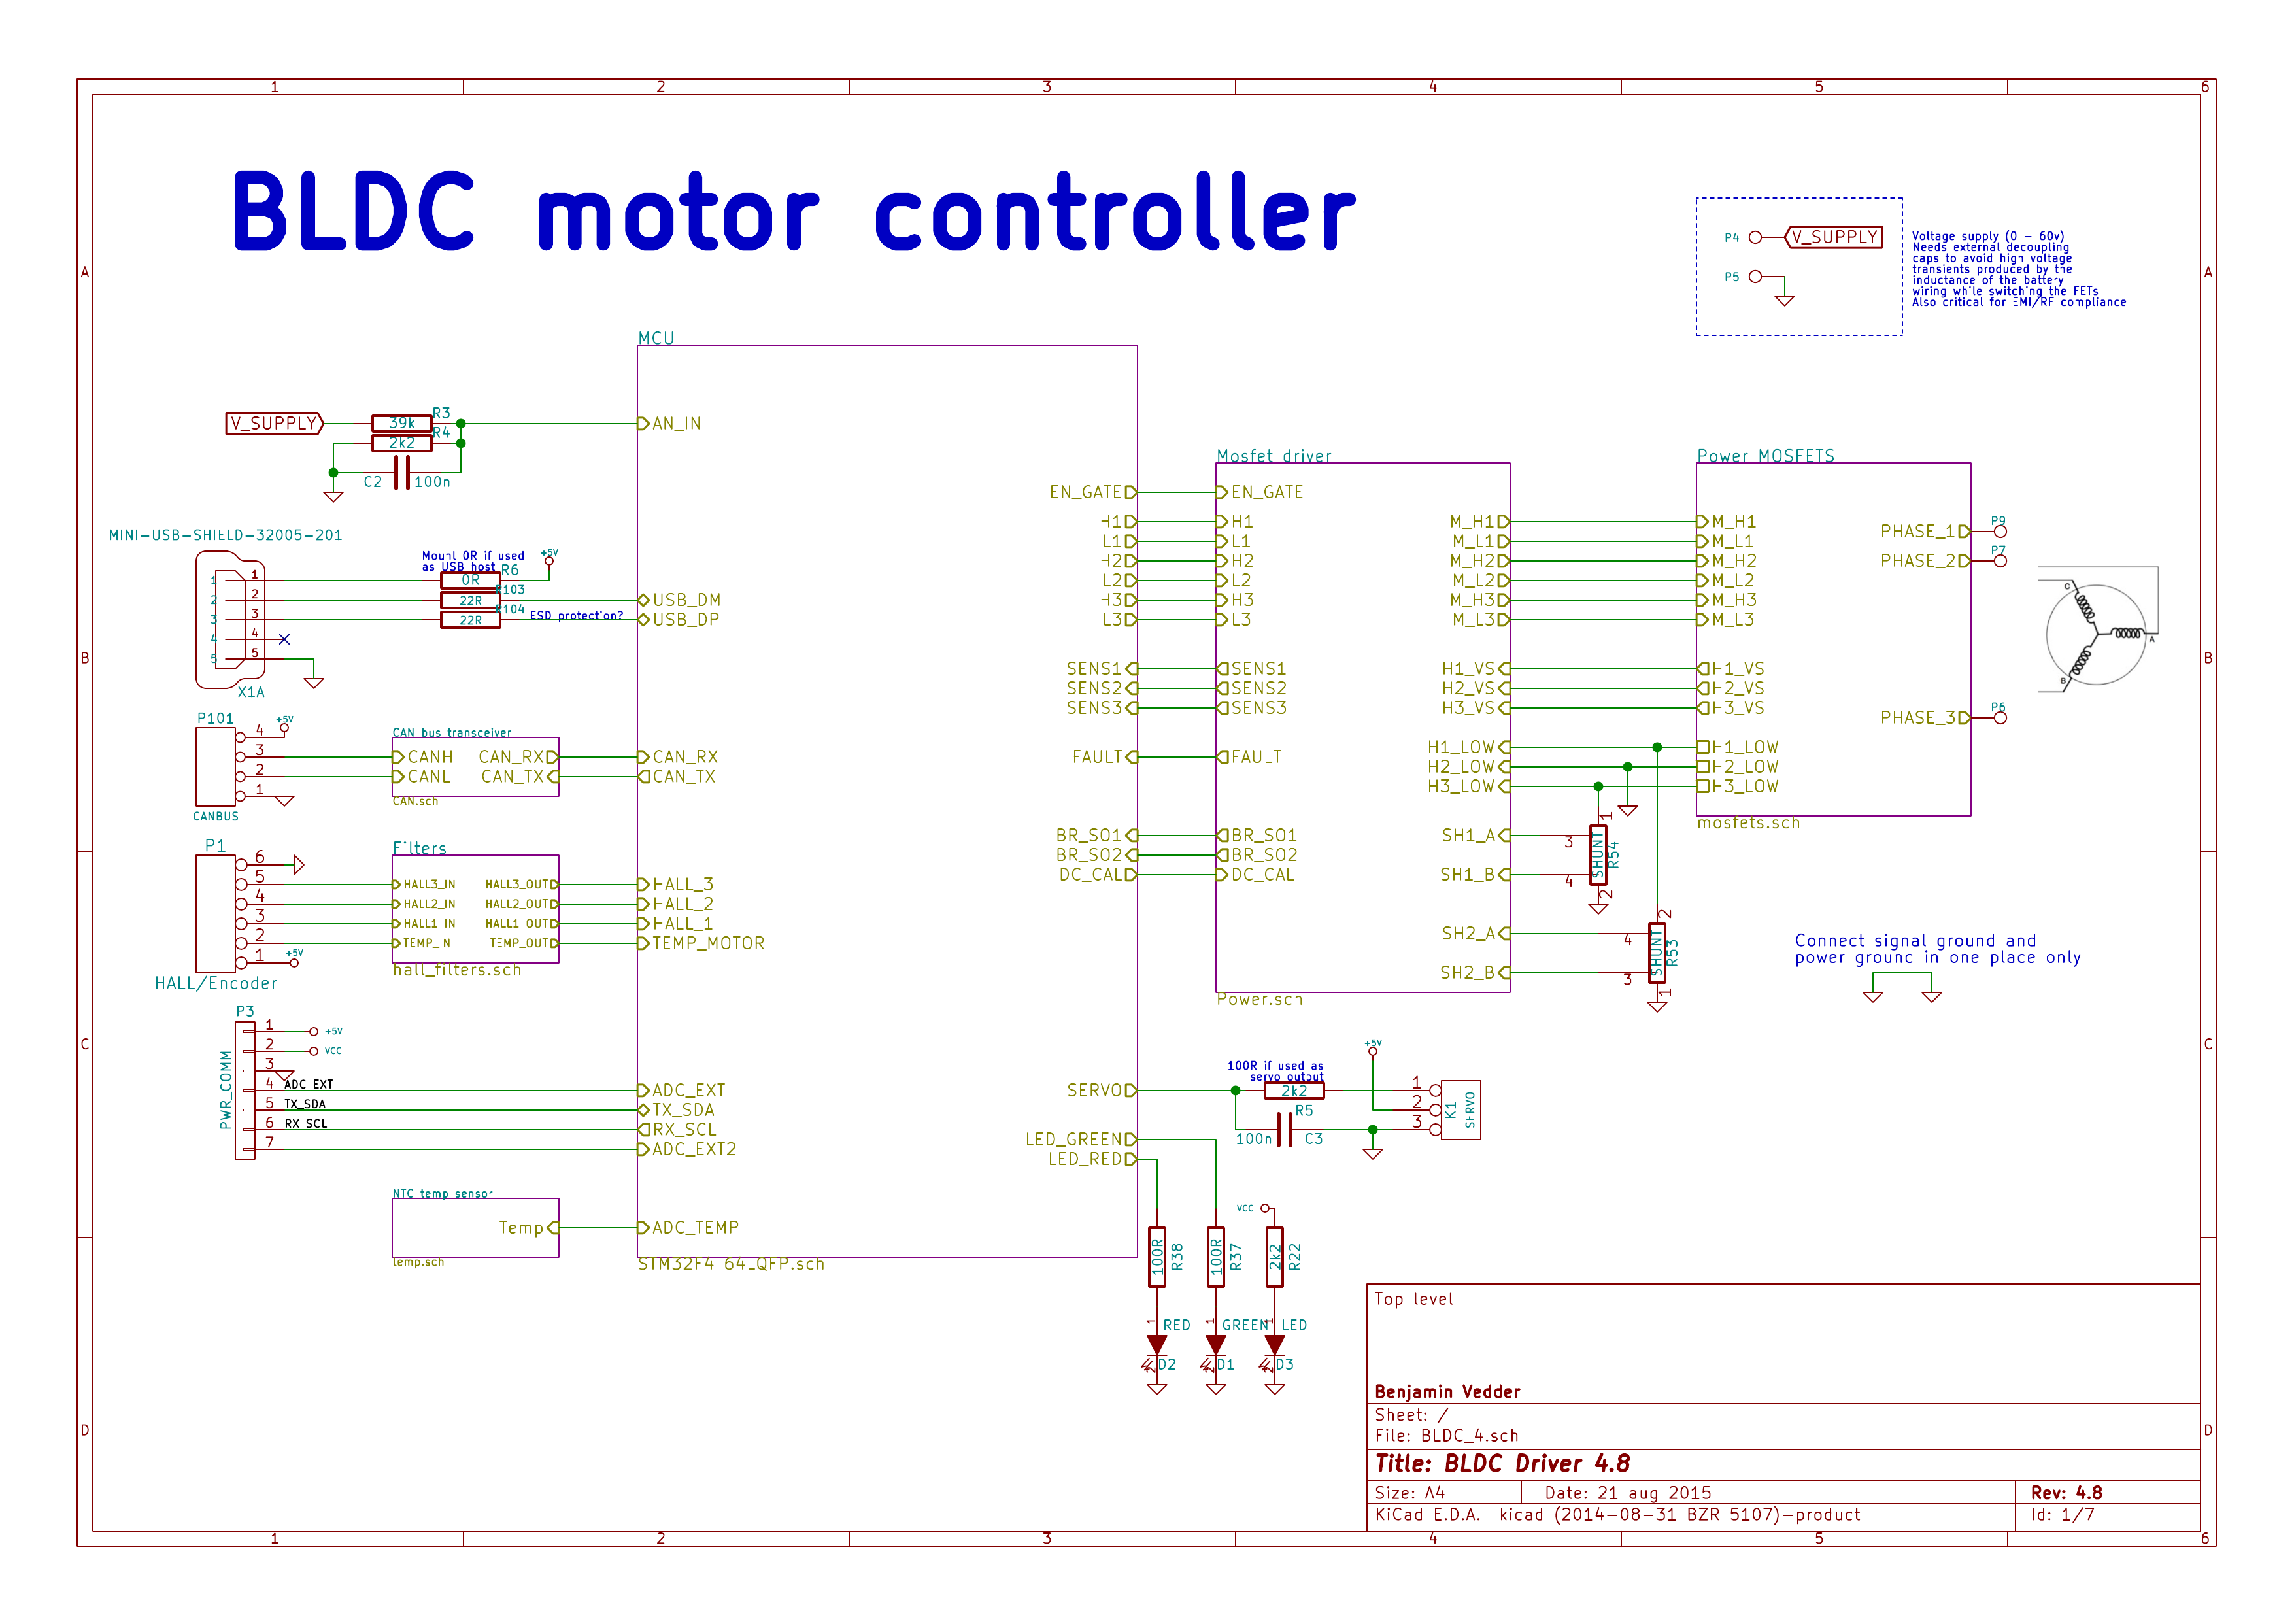
\includegraphics[width=\textwidth]{VESC/Schematic-1}
       
Podem observar que tenim el microcontrolador encapsulat amb el MCU i en el qual deriven senyals de diferents llocs. En aquests senyals depenent de com s'hagi configurat el firmware, es pot controlar el motor de diverses formes. Un cop hàgim realitzat els càlculs necessari passem el control dels mosfets de potència que rebran la informació del pont de transistors per activar o no les bobines necessàries.     
%podem oserver que tenim el micro encalusat amb el MCU i en el cual eriven senyasl de fiafrents llocs en quetes senyal depenent de com agem configura el frimware podem controlarlo el motor de difrentas formes, un coo agem realisat els calculs nasesaris pasem el control dels mosfets de potencia que rep informacio del pont de trensistors de trnesitors per activar o no les bonoines nesesaries
     
\subsection{Power mosfets}

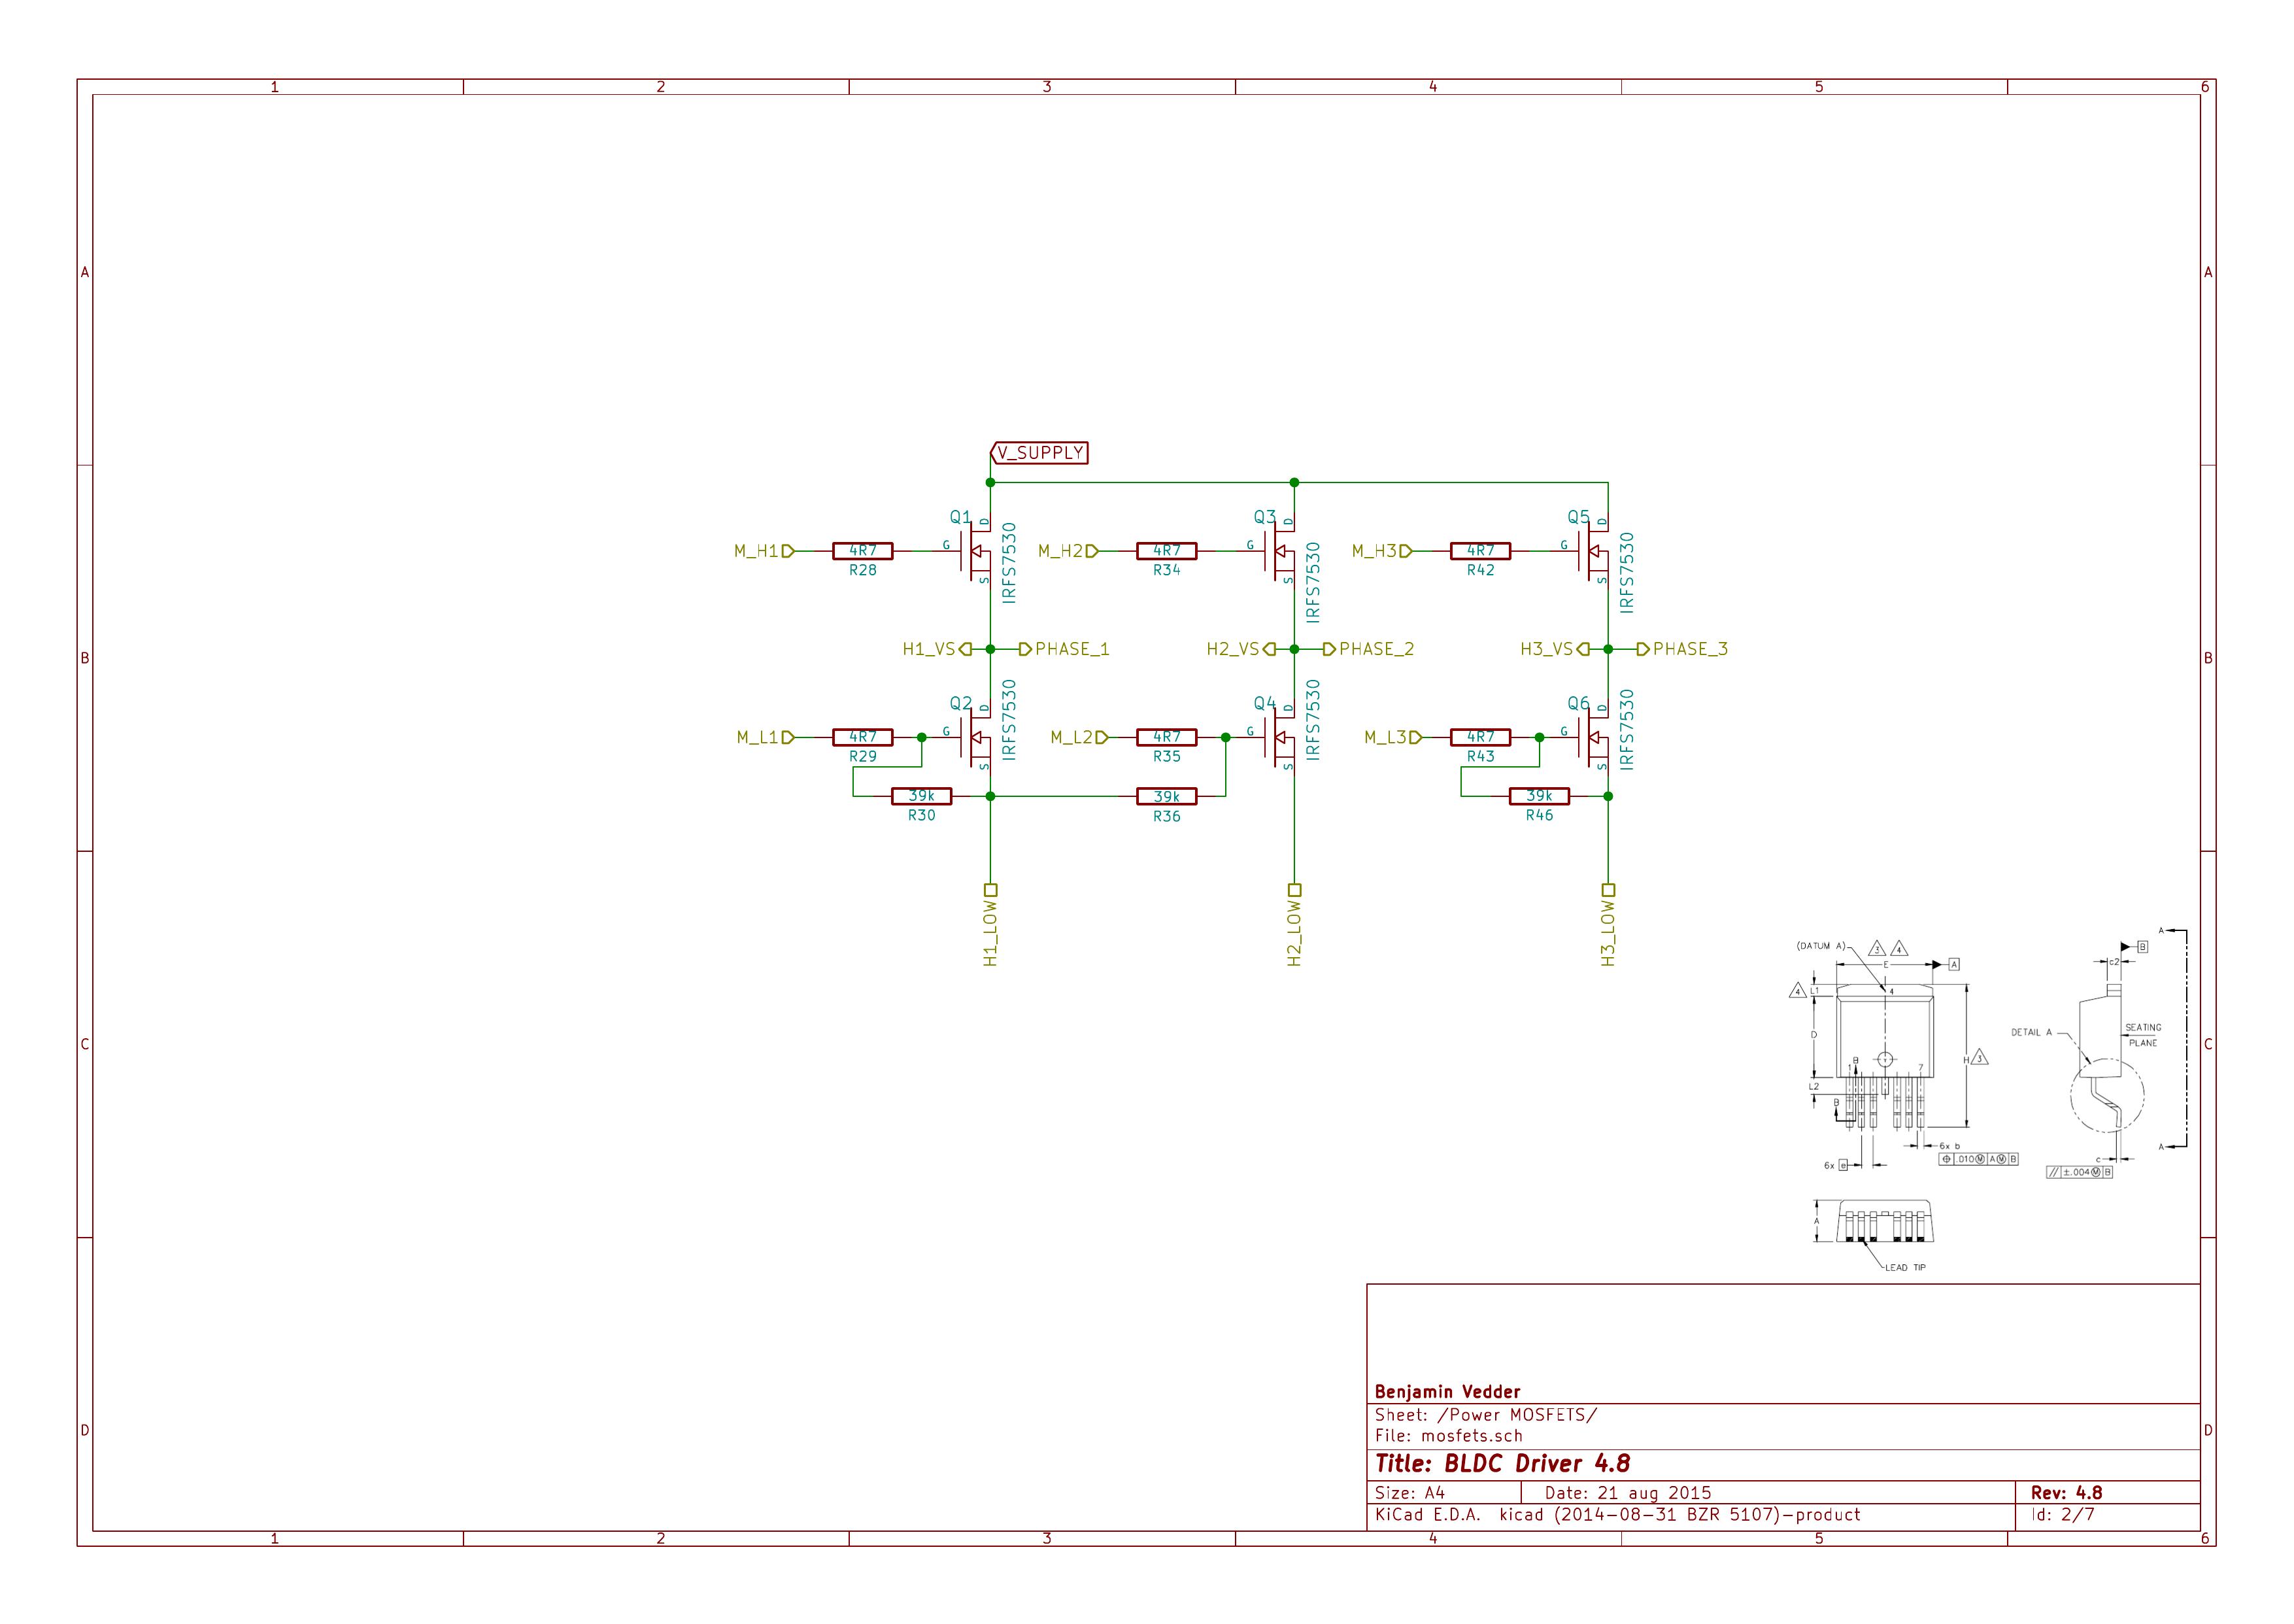
\includegraphics[width=\textwidth]{VESC/Schematic-2}
 
En la part dels mosfets tenim un triple pont en H per tal de poder generar les 3 fases que necessiten els motors brushless. També tenim els mesuradors de caiguda de voltatge en els mosfets per tal de poder detectar el curtcircuit en les diferents fases.
 
\subsubsection{Detecció de curtcircuit en l'inversor trifàsic}
 
 En un pont en H doble o triple si tenim el corrent que hi ha entre Vcc i el mig del pont. Podem detectar curtcircuits ja que el voltatge de caiguda que tindrem en el mosfet serà més elevat que el que tindríem si la potència passés per la bobina. Com sabem el mosfet proporciona un control resistiu, és a dir, podem canviar la seva resistència canviant la tensió entre la gate i el source. Això provoca un canvi de resistències entre el source i el drain. Sabent la tensió del source i la tensió del drain podem veure que tindríem una caiguda de tensió depenent de l'estat del mosfet. Si en la sortida hi hagués un curtcircuit, pràcticament tota la tensió es quedaria entre el source i el gate de forma que podem mesurar la intensitat de cada una d'elles. Podem observar unes resistències entre el gate i el source de forma que podem detectar-la i obrir el mosfet per no cremar-ho.
  
%\paragraph{detactar corciuquit en inversor trifaisc}
%en un pot en H doble o triple si tenim la corrent que hi ha entre el VCC i el mix del pont podem detactar corcirquits ja que el voltage de caijuda qur tindrem en el mosfet sera mes mes alavat que el que tindriam si la potencia pasa per la bobina, com saveme el mosfet proporciona un control resisitiu es a dir podem camviar la seva resistencia cavient la tensio entre el gate i el source, axo proboca un cavi de resistencia entre el source i el drain, si svem la tancio de la souce i la tencio del dran podem veure que tindrem una caiguda de tencio depeen del estat del mosfet, si en la surtida hi hages un corcicurut practiament tota la tencia escada entre el source i la gate de forma que podem detactarla i obrir el mosfet per no cremarlo.\smallskip 
     
També tenim les sortides de les branques separades per tal de poder mesurar la intensitat de cada una d'elles. Podem observar unes resistències entre la gate i el pin de tret per tal de limitar la intensitat que demanem al controlador.
%tambe tenim las sortides de las bracas separadas per tal de poder masurar la intenciat de cada una de ellas, podem obersar unses resisitecias entre ela gate i el pin de dispar per tal limitar la intencitat que demanem al controlador, 

\subsubsection{Intensitat del gate}
 En el gate d'un mosfet per norma general apareix un condensador. Això provoca que el tret del mosfet necessiti una intensitat per tal de carregar aquest condensador, si la intensitat no la limitéssim podríem cremar el control.
%\paragraph{intenciat en la gate} en las gsates del un mosfet per noma general aparex un capacitador aixo proboca que el dispar del el mosfet nenesisit una intenciatat per tal de carregar aquet capacitador si la intanciat que no la limitencim podriem crremar el control. 
     
\subsection{controlador del inversor}
En el VESC per dissenyar l'inversor trifàsic s'han basat en el xi DRV8302 per tal de controlar les 3 branques de pont en H:

\subsubsection{Descripció del DRV8302 }
L'integrat disposa d'unes entrades de control que permeten donar senyals als mosfets de potència per activar-los, de forma que ell eleva el voltatge i activa el mosfet. El mosfet ha d'estar a 5V entre gate i source, però el source en el moment de l'activació canvia de GND a VC menys la caiguda del mosfet. Si li apliquéssim 5V referenciats a massa no aconseguirem obrir el mosfet. Aquest integrat permet controlar tot aquest procés.

A part en permet capturar la mesura de corrent en dues de les fases, per tenir un control constant del corrent que fem circular pel motor i controlar el curtcircuit, just al moment en el qual el mosfet rep tota la caiguda de voltatge.

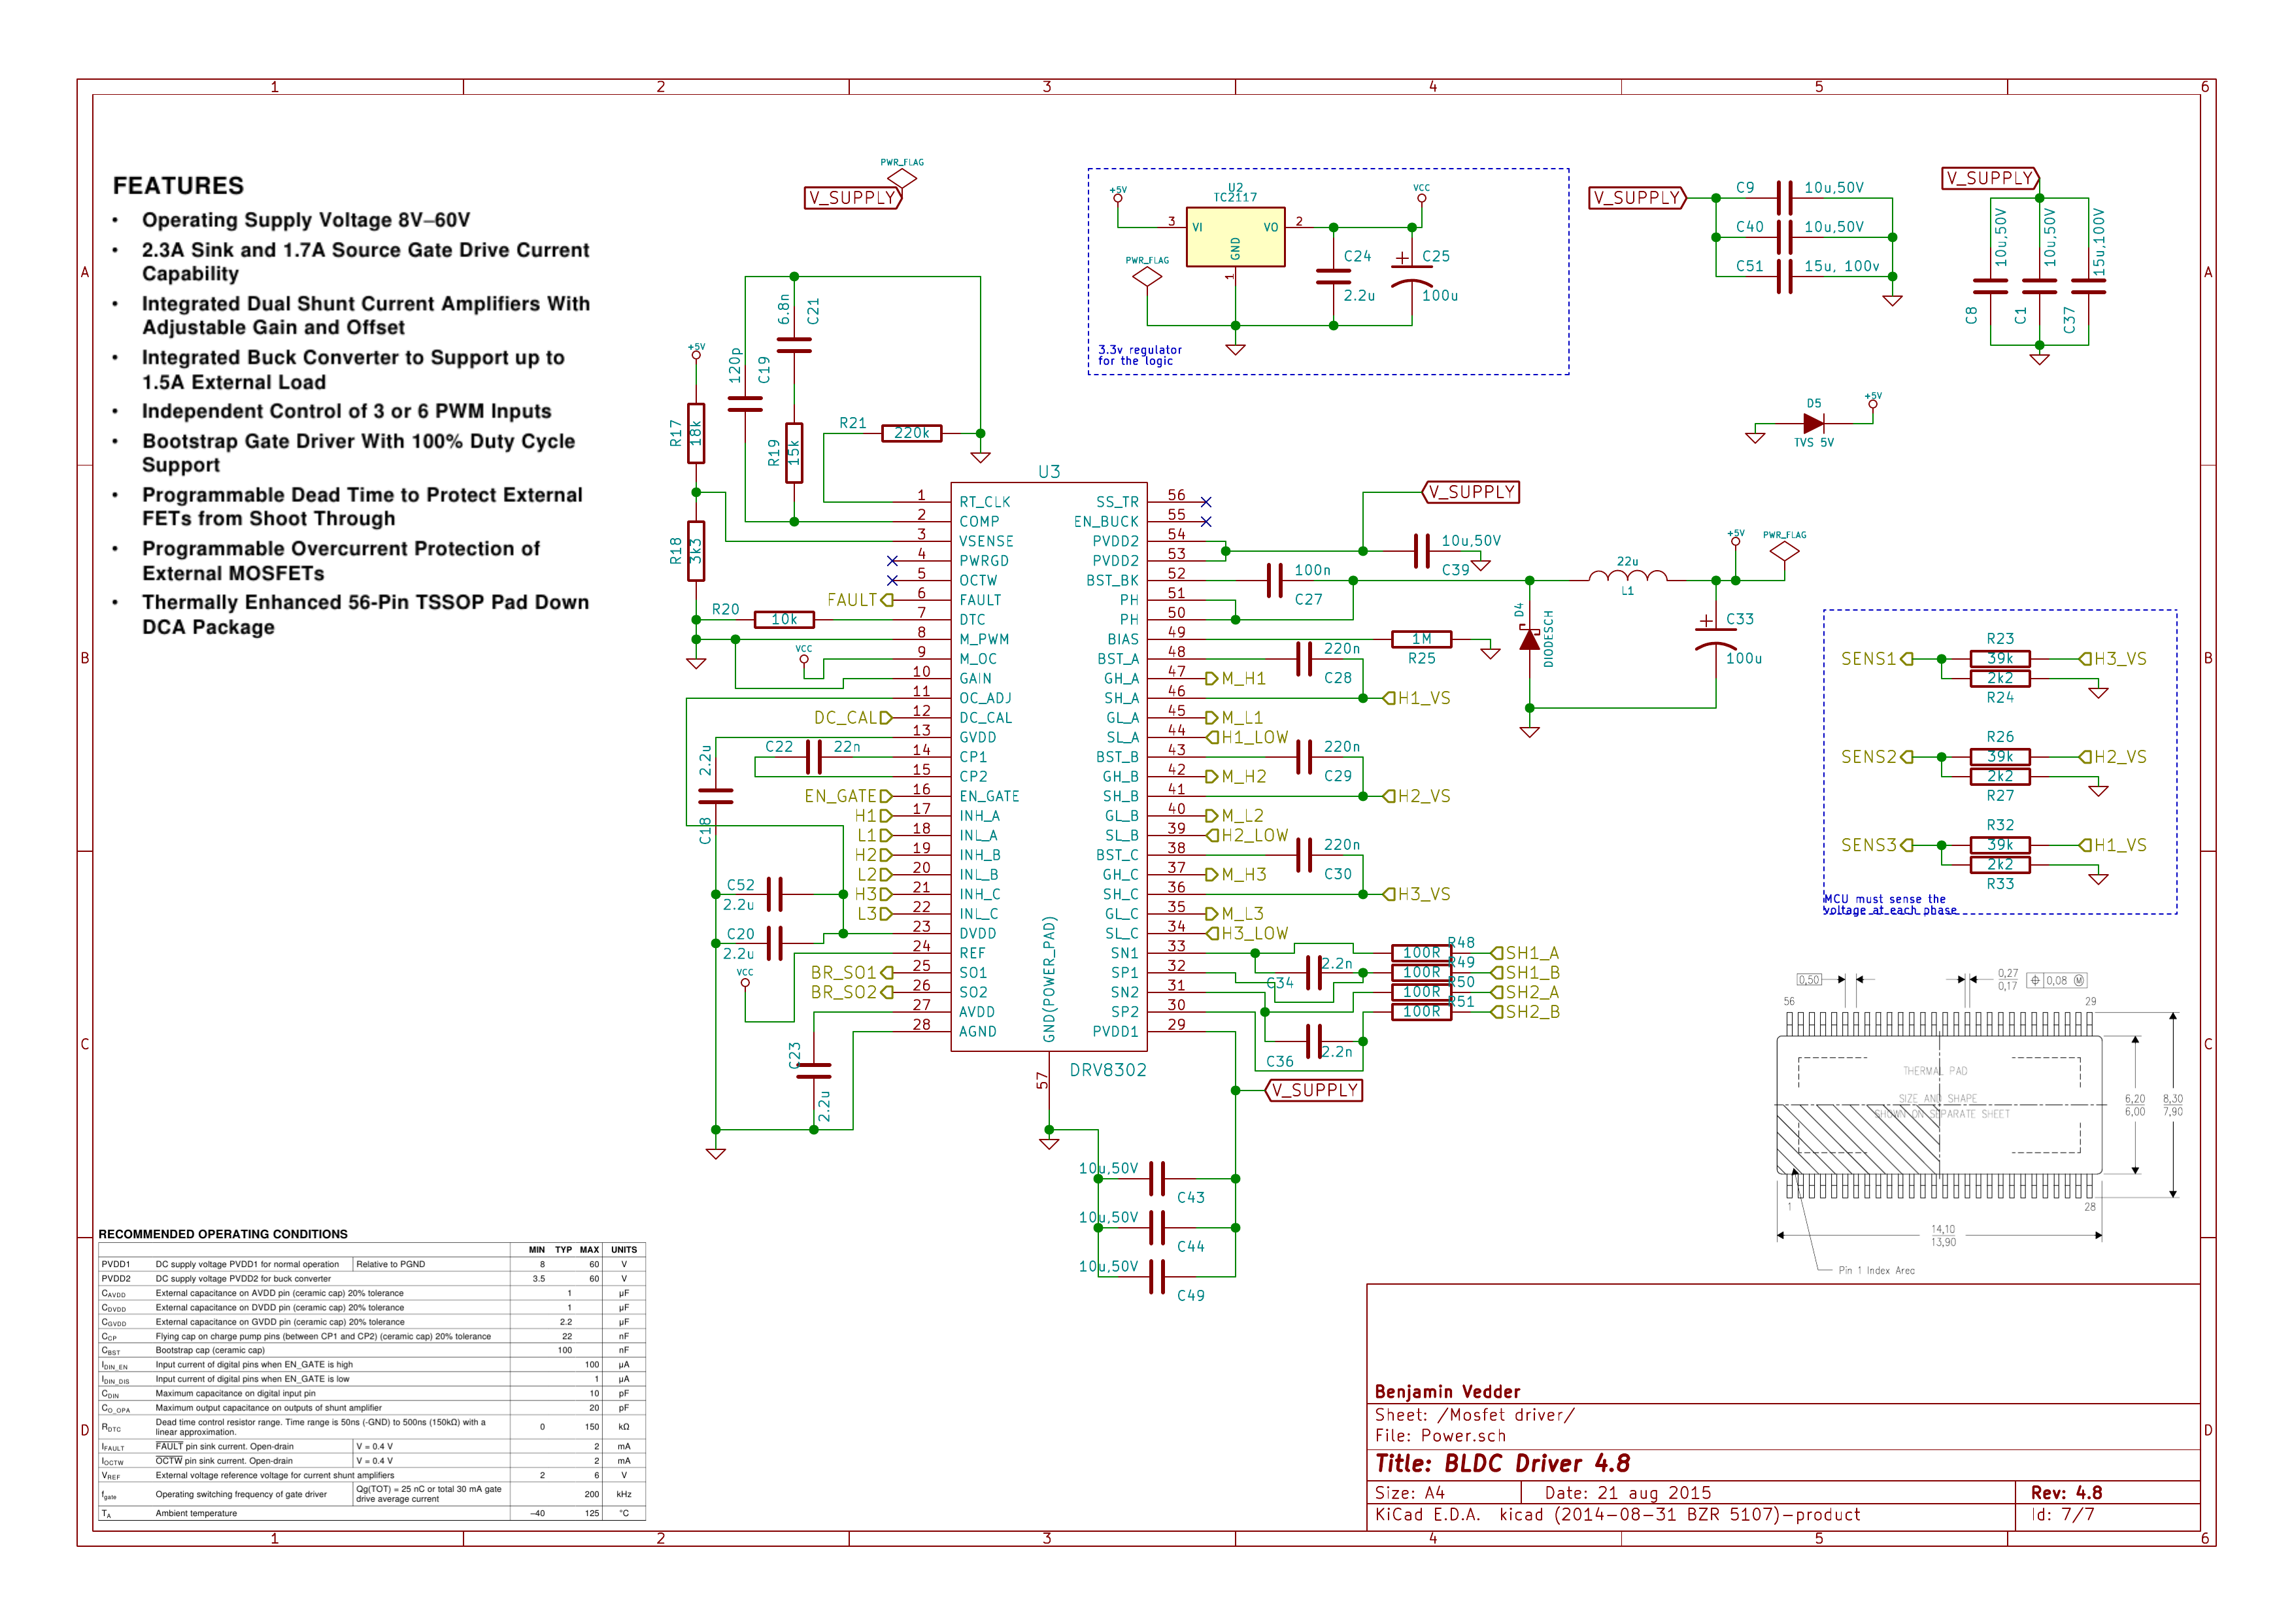
\includegraphics[width=\textwidth]{VESC/Schematic-7}

\subsection{Microcontrolador}
En el VESC disposem d'un microcontrolador capaç de controlar l'inversor trifàsic per tal d'adaptar-se a les característiques de software que tenim explicades. Aquest microcontrolador és un ARM CORTEX M4.

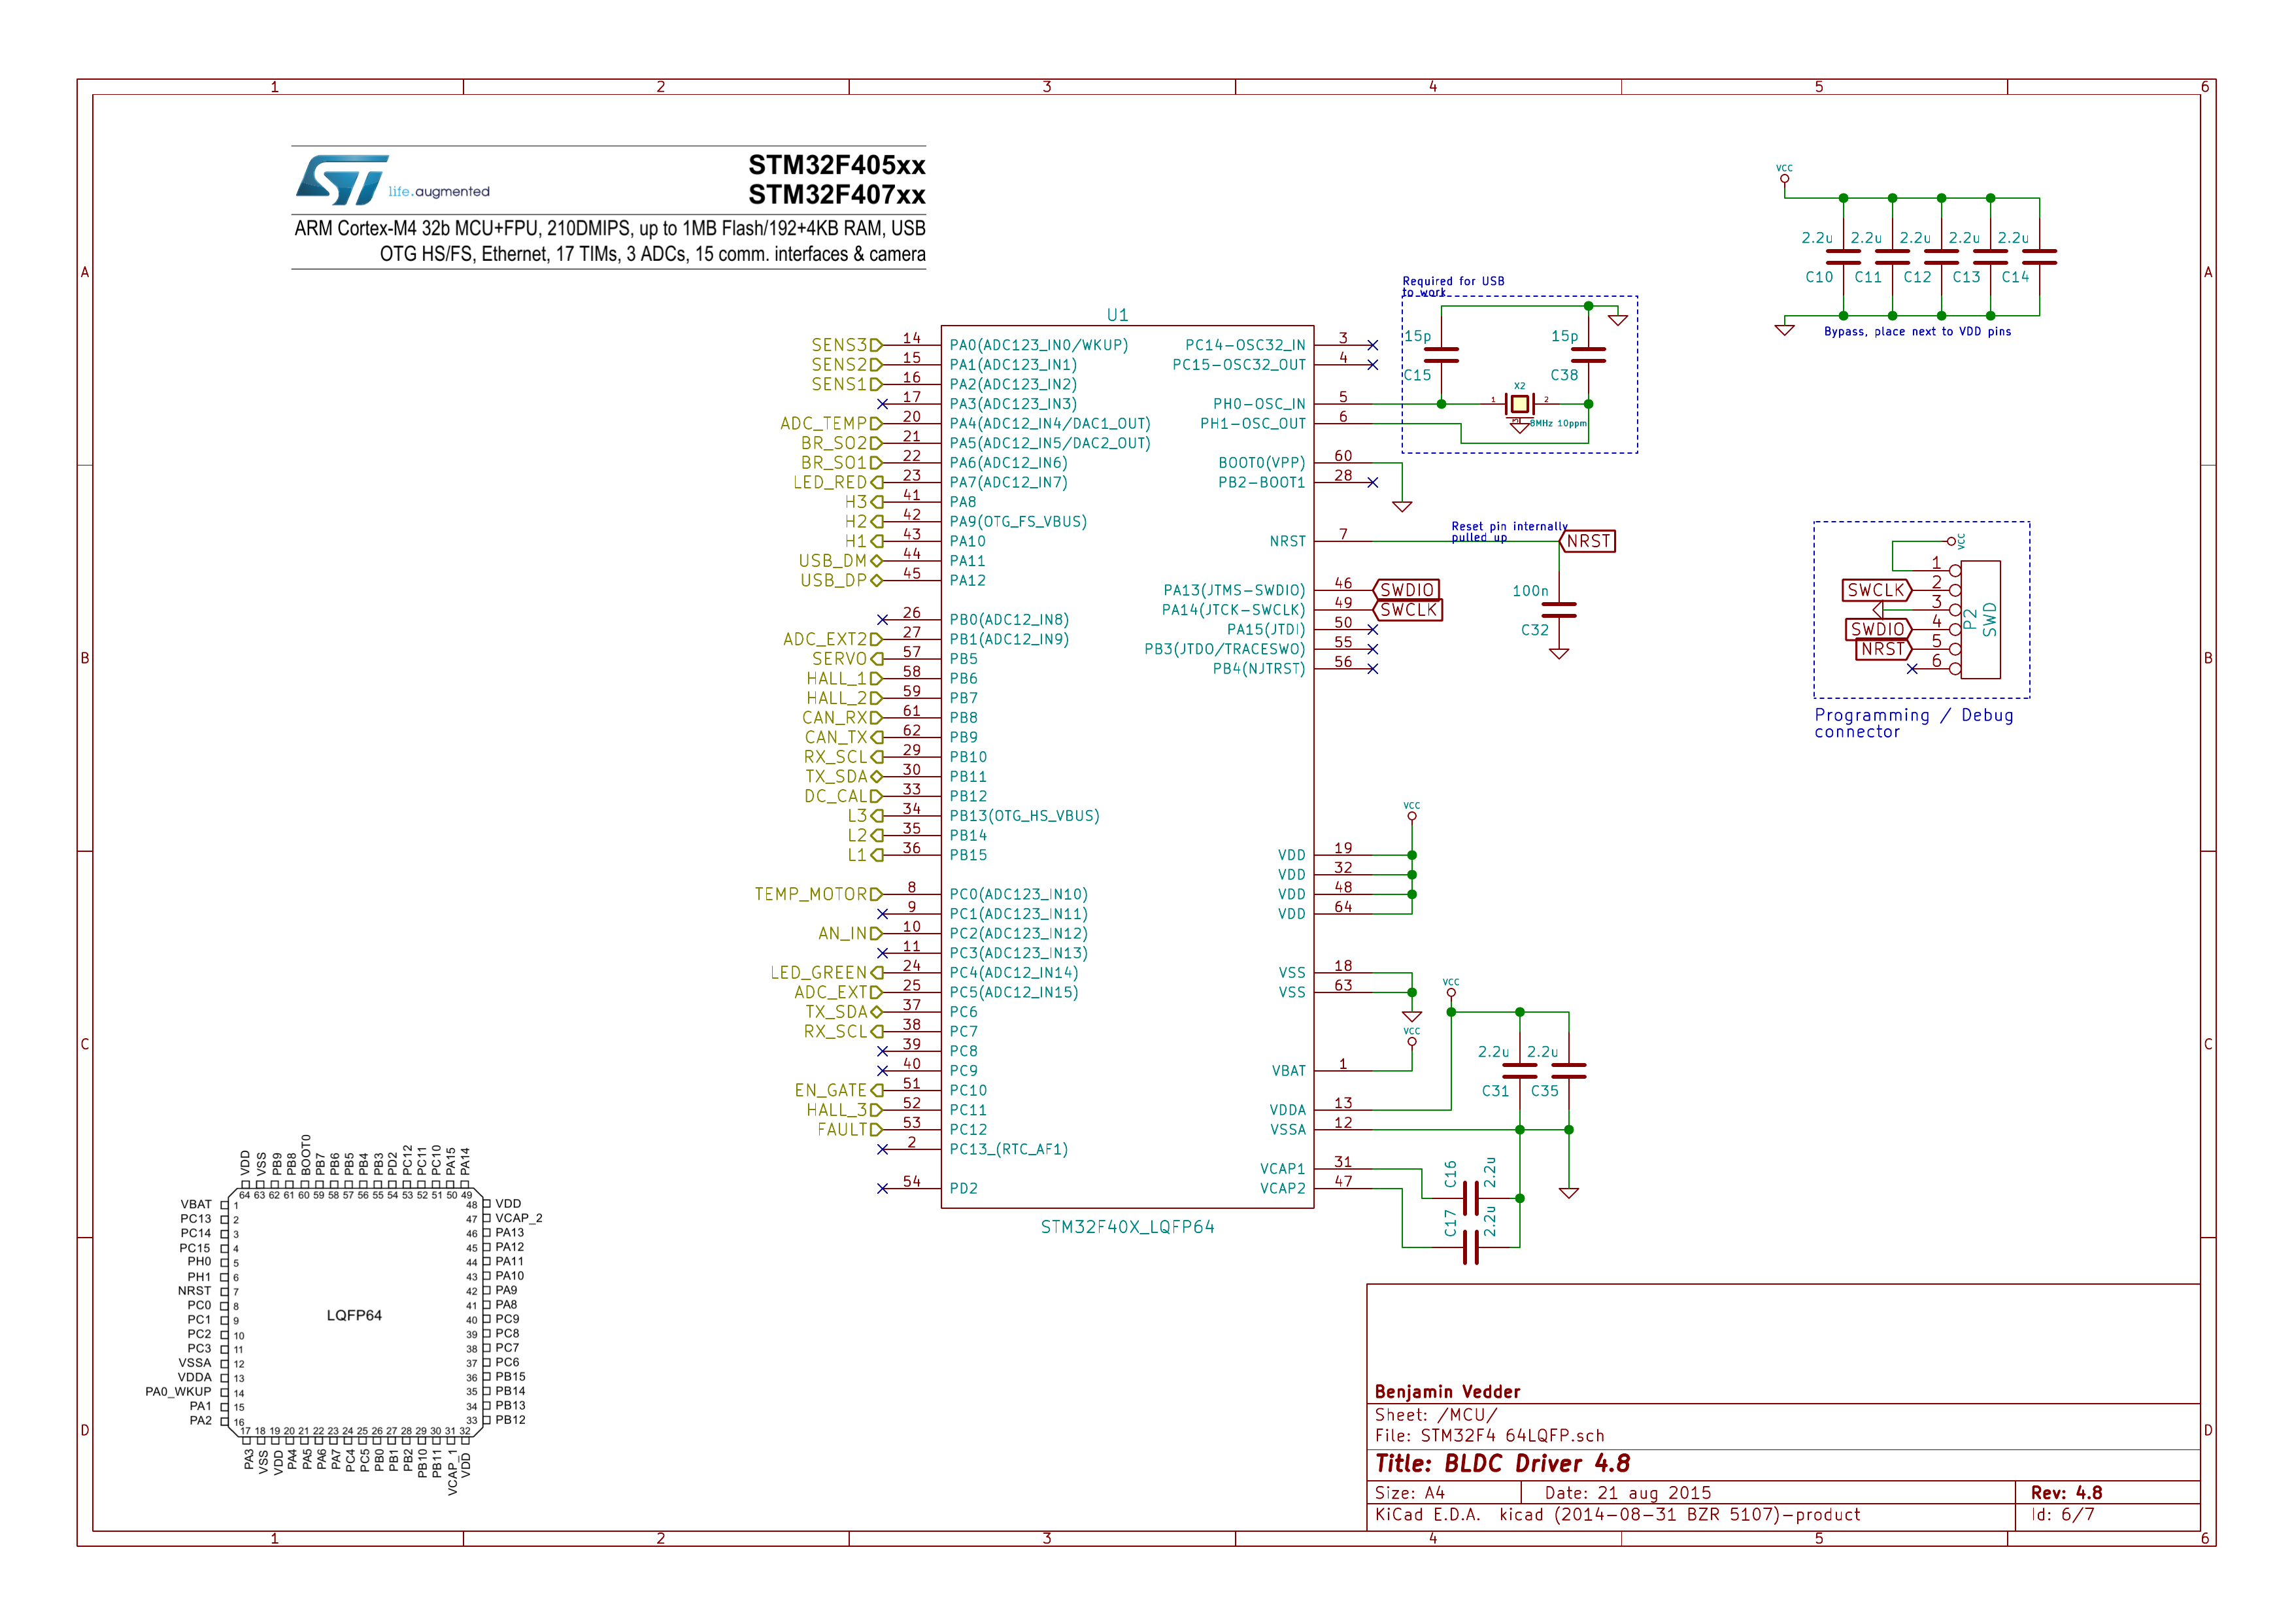
\includegraphics[width=\textwidth]{VESC/Schematic-6.png}
     
És un microcontrolador encarregat de controlar la major part del driver, des de les comunicacions fins al control de les oscil·lacions dels mosfets de potència. Per això disposarem de diversos comptadors, 17 de 15 de 16bits + 2 de 32 bits, per tal de generar les ones PWM o estar alerta en les comunicacions, entre altres funcions. Hi hauran diversos protocols de comunicacions tal com UART, I2C, CANBUS i SPI en un total de 15 ports, de forma que tindrem una gran capacitat d'adaptació a dispositius externs com comandaments o data-logers. A part disposem de dos Ethernet de 10/100 mbps per comunicacions avançades i usb, par tal de configurar-lo o capturar dades mitjançant computadors.\footnote{https://www.st.com/resource/en/datasheet/dm00037051.pdf}
     
\section{Algorismes de control}
Una vegada analitzat com està construït el controlador, anem a fer un repàs del codi del controlador. No serà un repàs exhaustiu del funcionament del firmware, però si poder veure una visió general de com funciona el control dels motors.
    
\subsection{Per què ens hem basat en el VESC}
És un dels pocs projectes d'aquest tipus que hi ha al mercat, però tot i així s'ha convertit en un referent i les marques privades l'utilitzen en els seus dispositius. A part poden analitzar el seu codi i entendre les funcions que fa per tractar d'implementar el nostre, modificar el VESC o decantar-no per utilitzar aquest controlador. A part he pogut analitzar una mica com està connectat i perquè està muntat com ho està, quins efectes apareixen al controlar motors en triple pont i que tenir en compte, coses que en l'electrònica explicada es tenien en compte ja que no tractàvem la potència.

\subsubsection{Efectes que apareixen el el pont en H}
En el control de motors de corrent continu els controlem amb el pont en H o el semipont en H. En aquest cas ens centrarem en el pont en H ja que és més similar al triple pont en H que és el que aplica el projecte.

\subsubsection{Pont en H en corrent continu}
En el moment que volem controlar un motor en els dos sentits controlant tant el corrent com el sentit d'aquest, és la selecció ideal.

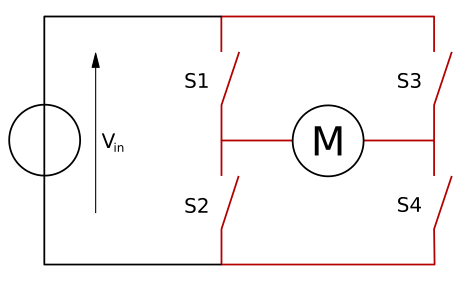
\includegraphics[width=\textwidth]{VESC/Hbritge.png}\bigskip
 
Depenent de la combinació de la commutació dels interruptors tenim diferents efectes. En el cas commutem S1 i S4 o S2 i S3 el motor girarà en un sentit o en l'altre, això provocarà que el corrent de la font vagi directament als pols del motor i provoqui la màxima potència en algun dels sentits. Si el control es realitza per pulsacions PWM podem controlar el corrent que li enviem al motor per tal de fer que funcioni a mig gas o com vulguem. 
 
S'ha de tenir en compte l'efecte que ha de deixar un motor girant amb el pols a l'aire, un motor girant és un generador de corrent, és a dir, que convertirà la seva energia cinètica en corrent que s'acumularà als pols del motor. Això pot provocar un pic de sobrecorrent en el transistor que controla el pont. S'han de muntar díodes de descàrrega en sentit oposat o mantenir els interruptors activats per tal de drenar el corrent generat pel motor.

Si en algun moment volem efectuar una parada ràpida del motor, podem jugar alimentant el motor en sentit contrari, en el cas que el control ho permeti, o podrem curtcircuitar els seus pols per tal de provocar un curtcircuit i fer desaccelerar el motor ràpidament. Això ho faríem activant S1 i S3 o S2 i S4 de forma que el corrent generat circuli per la part superior o inferior del pont.

\subsubsection{Rectificador trifàsic en CC}
El rectificador trifàsic és el mateix que el pont en H però afegint una branca més per poder treure les 3 fases.

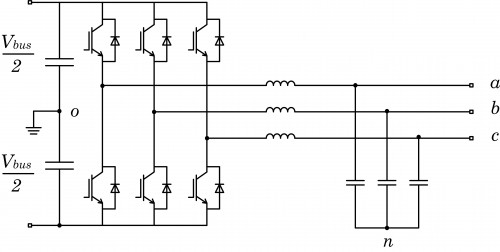
\includegraphics[width=\textwidth]{ilustracion-1-13281.jpg}\bigskip

Tenim el mateix que en el pont en H però amb una tercera branca. En el cas del rectificador trifàsic normalment es poden afegir uns filtres de corrent i voltatge a les bobines i codificar per tal d'estabilitzar l'ona generada ja que el control serà per polsos. Tant el voltatge com el corrent seran polsants, d'aquesta manera podríem filtrar harmònics que podrien ser no desitjats, depenent de com commutin S1, S2 i S3 (superiors) i S4, S5 i S6 (inferiors) podríem crear la forma d'ona i la freqüència desitjada per tal d'enviar-la al rectificador.
%tenim el matex que el pont en H per amb una tercera branca, en el cas del trectificafot trifaisc normalemnt es poden afagir un filtres de corrtent i volatrga, bobines i condececodr per tal de entabilisar la ona generada ja que el control sera per pulsos i tan el voltatge i el cotrent sera pulsat, de aquenta menre podriem filtrar armonics que podrien ser no desigats, depenent de com comuent s1 s2 s3 (superiors) i s4 s5 i s6 (inferiors) podriem crear la forma de ona i la frecuencida desitgada per tal de enviar al rectificador.\medskip

També cal tenir en compte que volem controlar motors brushless i el seu control és com el d'un motor CC, amb la diferència que tenen 3 fases i per tant els filtres no serien necessaris i podrien molestar ja que tot filtre provoca retards i no seria útil en el nostre cas.

\section{aspectes a teir en conte}
Una vegada repassat com funciona el control dels motors brushless per vehicles elèctrics ens adonem que en el control tenim molts aspectes que influeixen com pot ser la freqüència de commutació, la fase del motor, la freqüència de l'ona generada i la posició del roto, com plantegem cada una d'aquestes característiques i com les controlem.

\subsubsection{Freqüència de commutació}

Si podem controlar la freqüència de commutació dels transistors podrem millorar l'eficiència de l'inversor trifàsic, és a dir, a una menor freqüència les pèrdues de commutació seran menors i el corrent que li arribarà al motor tindrà un menor soroll. suposem que volem generar polso quadrats a una freqüenta de 1khz en el 80/100 del voltege per tal de controlar el motor, si el nostre pwm commuta a 500khz el que ens trobarem es que commutem moltíssimes vagades, axó provocarà sobreescalfament en el mosfets, ja que dissipen molta més potencia en commutació, i un soroll molt important en el motor, per tal si vexem la frecuancia de commutació a 100khz, podríem generar la mateixa ona però amb 400 comunicacions menos per segons el que milloraria la eficacia

% CURT? AQUI COMENTAM AVIAM SI AFEGIRAS MES O QUE FARAS, SINO POTSER FAIG UN APAÑO

\section{Selecció del control desitjat i modelació de la PCB}

Per tal de poder adaptar el nostre sistema al VESC necessitaríem fer unes millores en l'electrònica i una modificació del firmware per tal de suportar voltatges més alts deguts a la complicació que tenim a l'hora de controlar el ponts en H. Això és una feina que ja vam provar amb una complexitat molt elevada.
